\title[EG \LaTeX\ Author Guidelines]%
      {Volumetric Ray Tracing}

% for anonymous conference submission please enter your SUBMISSION ID
% instead of the author's name (and leave the affiliation blank) !!
\author[Matthias Eberhardt]
%{\parbox{\textwidth}{\centering D.\,W. Fellner\thanks{Chairman Eurographics Publications Board}$^{1,2}$
 %      and S. Behnke$^{2}$
 {\parbox{\textwidth}{\centering Matthias Eberhardt$^{1}$
%        S. Spencer$^2$\thanks{Chairman Siggraph Publications Board}
        }
        \\
% For Computer Graphics Forum: Please use the abbreviation of your first name.
{\parbox{\textwidth}{\centering $^1$OTH Regensburg, Germany
%        $^2$ Another Department to illustrate the use in papers from authors
%             with different affiliations
       }
}
}
% ------------------------------------------------------------------------

% if the Editors-in-Chief have given you the data, you may uncomment
% the following five lines and insert it here
%
\volume{2021}   % the volume in which the issue will be published;
\issue{1}     % the issue number of the publication
% \pStartPage{1}      % set starting page


%-------------------------------------------------------------------------
\begin{document}


\maketitle
%-------------------------------------------------------------------------
\begin{abstract}
  This paper presents an overview of several methods used for volumetric rendering.
\end{abstract}  
%-------------------------------------------------------------------------

\section{Introduction}

Volumetric ray tracing is well suited for rendering 3-dimensional objects, which cannot be easily represented as a set of geometric primitives, e. g. clouds~\cite{10.1145/964965.808594}.

\section{Classical Ray Tracing Equation}




\section{Modification Of The Ray Tracing Equation For Volume Rendering}

%-------------------------------------------------------------------------


\begin{figure}[htb]
  \centering
  % the following command controls the width of the embedded file
  % (relative to the width of the current column)
  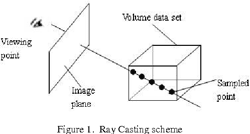
\includegraphics[width=.8\linewidth]{RayCasting1.png}
  \parbox[t]{.9\columnwidth}{\relax }~\cite{Appa2015RayCF}
  %
  \caption{\label{fig:firstExample}
          Illustration of the ray casting process.}
\end{figure}



\bibliographystyle{plain}
\bibliography{mybib}



%-------------------------------------------------------------------------
% bibtex
%\bibliographystyle{eg-alpha-doi} 
%\bibliography{bib}       

% biblatex with biber
%\printbibliography                

%-------------------------------------------------------------------------


